\chapter{Additional Results}\label{app:embeddings}

\Cref{fig:app:emb_joint} shows \gls{umap} projections of the Vanilla joint encoder and the matching single-task run on two test windows, the same models as \cref{sec:exp:ablation}.
Window $100$ has two emitters and two modes; window $400$ has five emitters and nine modes.
Both columns recover the partitions on these windows.
The figure is included for inspection of the geometry; scores remain those of \cref{tab:exp:ablation_loss,fig:exp:kcorr_ablation_em,fig:exp:kcorr_ablation_md}.

\begin{figure}[p]
  \centering
  \IfFileExists{figures/experiments/emb_vanilla_joint_vs_separate.pdf}{%
    
\includegraphics[width=\linewidth,height=0.86\textheight,keepaspectratio]{experiments/emb_vanilla_joint_vs_separate.pdf}%
  }{%
    \IfFileExists{../../figures/experiments/emb_vanilla_joint_vs_separate.pdf}{%
      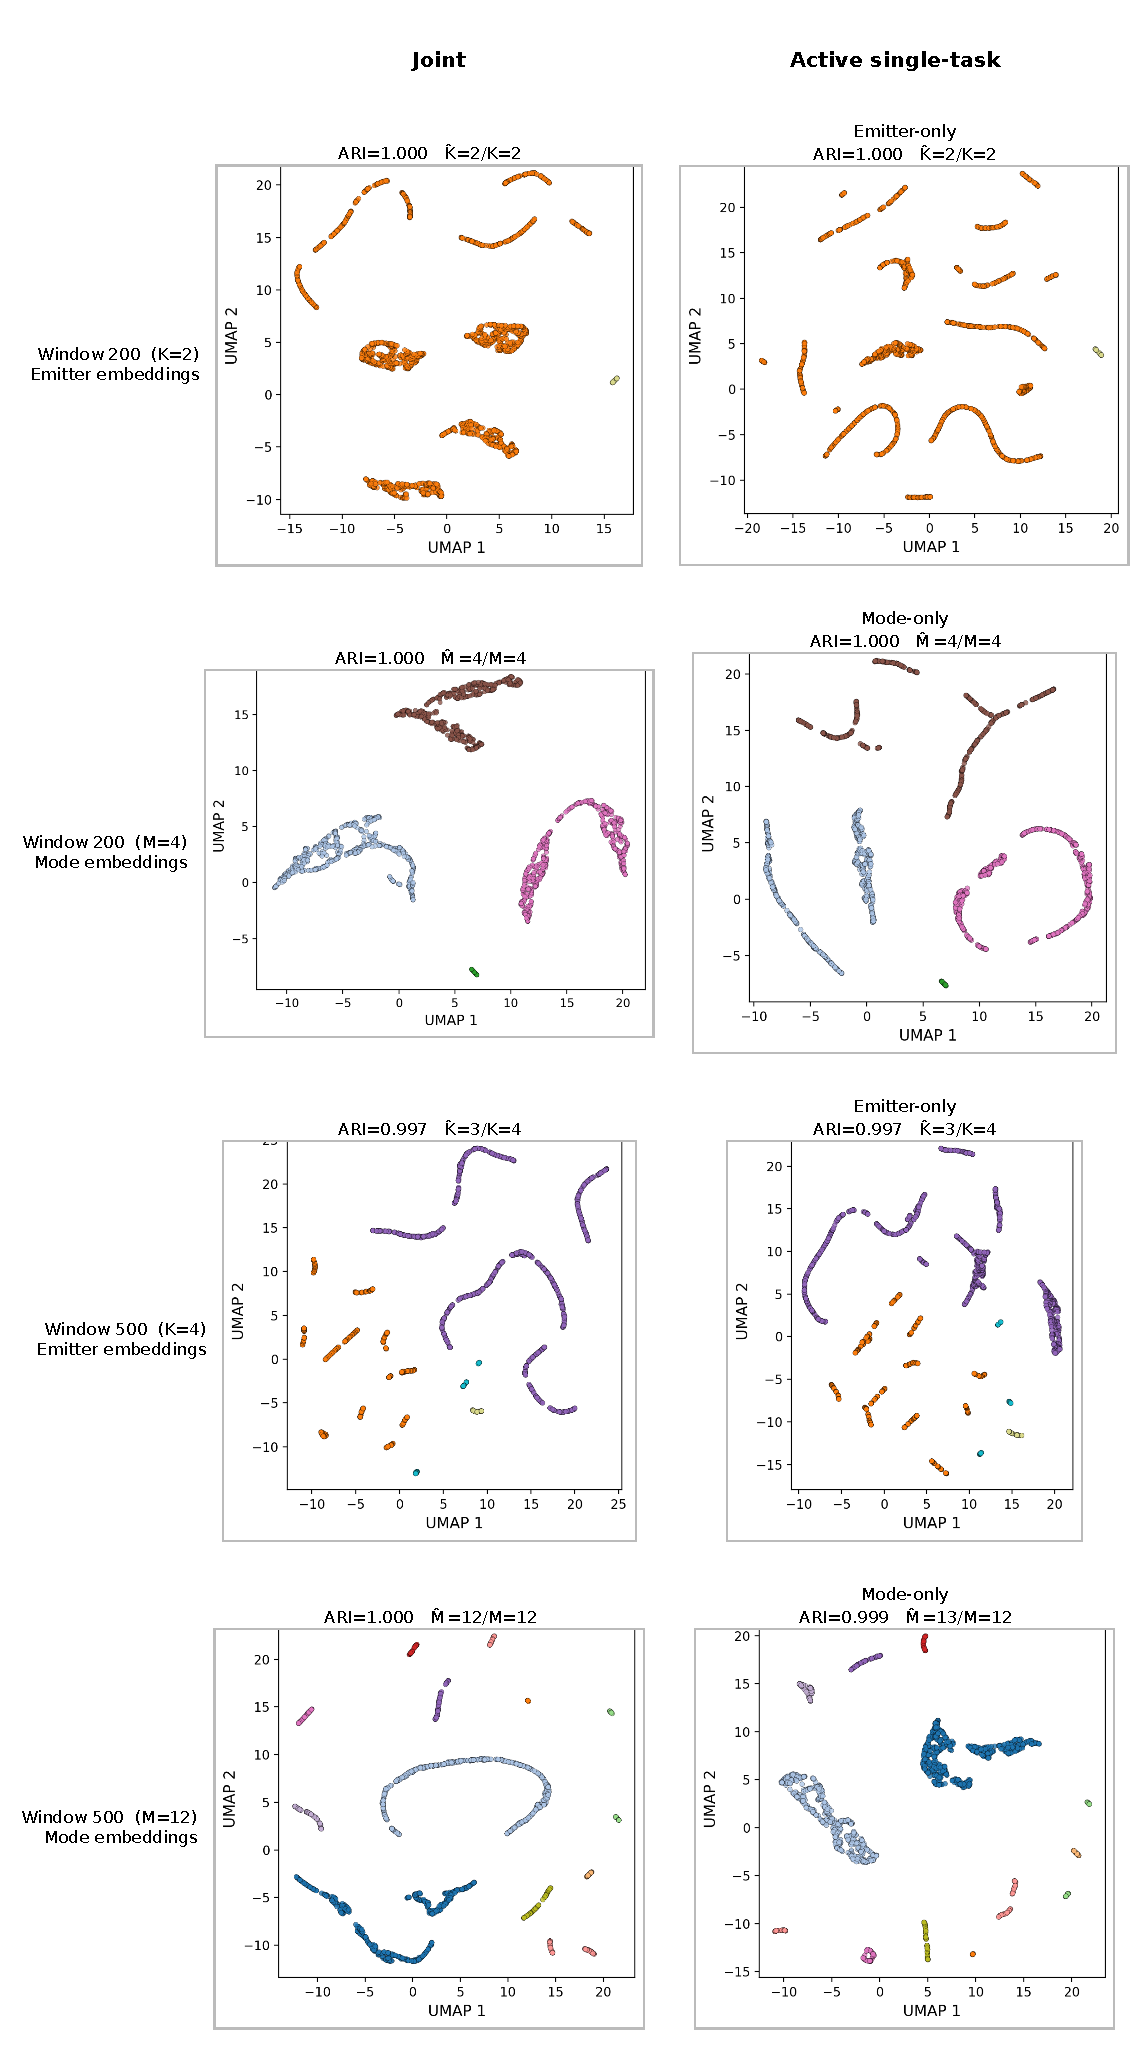
\includegraphics[width=\linewidth,height=0.86\textheight,keepaspectratio]{../../figures/experiments/emb_vanilla_joint_vs_separate.pdf}%
    }{%
      \expfig{emb_vanilla_joint_vs_separate.pdf}%
    }%
  }
  \caption{UMAP of active-branch embeddings on two test windows, colored by ground-truth labels. Columns are Joint and the matching single-task run. Rows alternate emitter and mode embeddings. Window $100$ has $K=2$ and $M=2$; window $400$ has $K=5$ and $M=9$.}
  \label{fig:app:emb_joint}
\end{figure}

\subsection*{All-model $\ARI$ comparison}\label{app:ari_all}

\Cref{tab:app:ari_em,tab:app:ari_md} collect mean per-window $\ARI$ for every encoder in \cref{ch:experiments}, including the single-task runs of Vanilla, RoPE-TOA, and Bias.
RoPE-az and RoPE-TOA+Bias have no single-task copy among the trained encoders.
Single-task rows report the active branch only.
Feature \gls{dbscan} is the no-encoder control of \cref{tab:exp:vanilla}.
Joint rows are copied from \cref{tab:exp:attn_em,tab:exp:attn_md,tab:exp:ablation_loss}, not from a second evaluation.

On the emitter branch, Emitter-only Vanilla, joint RoPE-TOA, emitter-only RoPE-TOA, and joint Bias sit at the ceiling.
Emitter-only Bias does not: its mean $\ARI$ is $0.840$, in the same band as joint RoPE-TOA+Bias.

On the mode branch every neural run occupies a narrow band.
Bias (Joint) is highest.
Mode-only Vanilla, RoPE-TOA, and Bias stay within rounding of their joint copies.

\Cref{fig:app:hist_em_all,fig:app:hist_md_all} are the matching empirical CDFs, on the same log vertical axis as \cref{fig:exp:hist_em,fig:exp:hist_md}.
Dashed curves are single-task runs.
The emitter plot makes the Bias emitter-only tail visible: it leaves zero with RoPE-TOA+Bias, while emitter-only Vanilla and both RoPE-TOA curves stay down until just below $1$.
Emitter-only RoPE-TOA has two windows below $0.50$, which the mean in \cref{tab:app:ari_em} does not show.
The mode curves rise later and closer together.

\begin{table}[H]
  \centering
  \small
  \caption{Emitter $\ARI$ on the test split for every trained encoder and Feature \gls{dbscan}. Single-task rows are the active branch. Entries are mean $\pm$ std over windows.}
  \label{tab:app:ari_em}
  \begin{tabular}{@{}llc@{}}
    \toprule
    Model & Objective & $\ARI$ \\
    \midrule
    Feature DBSCAN & {---} & $0.578\pm0.348$ \\
    Vanilla & Joint & $0.948\pm0.176$ \\
    Vanilla & Emitter-only & $0.999\pm0.012$ \\
    RoPE-TOA & Joint & $\mathbf{1.000\pm0.003}$ \\
    RoPE-TOA & Emitter-only & $0.998\pm0.036$ \\
    RoPE-az & Joint & $0.973\pm0.135$ \\
    Bias & Joint & $\mathbf{1.000\pm0.002}$ \\
    Bias & Emitter-only & $0.840\pm0.265$ \\
    RoPE-TOA+Bias & Joint & $0.851\pm0.255$ \\
    \bottomrule
  \end{tabular}
\end{table}

\begin{table}[H]
  \centering
  \small
  \caption{Mode $\ARI$ on the same windows as \cref{tab:app:ari_em}. Single-task rows are the active branch.}
  \label{tab:app:ari_md}
  \begin{tabular}{@{}llc@{}}
    \toprule
    Model & Objective & $\ARI$ \\
    \midrule
    Feature DBSCAN & {---} & $0.811\pm0.250$ \\
    Vanilla & Joint & $0.985\pm0.107$ \\
    Vanilla & Mode-only & $0.983\pm0.110$ \\
    RoPE-TOA & Joint & $0.991\pm0.075$ \\
    RoPE-TOA & Mode-only & $0.984\pm0.100$ \\
    RoPE-az & Joint & $0.983\pm0.102$ \\
    Bias & Joint & $\mathbf{0.992\pm0.081}$ \\
    Bias & Mode-only & $0.981\pm0.117$ \\
    RoPE-TOA+Bias & Joint & $0.977\pm0.112$ \\
    \bottomrule
  \end{tabular}
\end{table}

\begin{figure}[H]
  \centering
  \expfig{hist_em_all.pdf}
  \caption{Empirical CDF of emitter $\ARI$ for every trained encoder, including single-task runs of Vanilla, RoPE-TOA, and Bias. The vertical axis is logarithmic. Layout follows \cref{fig:exp:hist_em}.}
  \label{fig:app:hist_em_all}
\end{figure}

\begin{figure}[H]
  \centering
  \expfig{hist_md_all.pdf}
  \caption{Empirical CDF of mode $\ARI$ over the same windows as \cref{fig:app:hist_em_all}. Dashed curves are mode-only runs.}
  \label{fig:app:hist_md_all}
\end{figure}
